%!TEX program = xelatex
%\documentclass[cn,hazy,blue,14pt,screen]{elegantnote}

\documentclass[cn,normal,11pt,blue]{elegantnote}
\usepackage{epsfig,amssymb,amsmath,version}
\usepackage{amssymb,version,graphicx,fancybox,mathrsfs,multirow}
%\usepackage[notcite,notref]{showkeys}
\usepackage{fontspec}
\usepackage{diagbox}
\usetikzlibrary{arrows,shapes}


\usepackage{tocloft}
\renewcommand{\cfttoctitlefont}{\hfill \bfseries \LARGE}
\renewcommand{\contentsname}{\centerline{\color{ecolor}目~~录}}
\renewcommand{\cftaftertoctitle}{\hfill}
\setlength{\cftbeforetoctitleskip}{10ex}
\setlength{\cftaftertoctitleskip}{5ex}
\renewcommand{\cftsecdotsep}{\cftdotsep}  % 设置Section引导点
\renewcommand{\cftbeforesecskip}{3ex}
\renewcommand{\cftbeforesubsecskip}{1ex}
% \renewcommand{\cftsecfont}{\songti}   % 设置Section字体



%%%%%%%%%%%%%%%%%%%%%%%%% Code Style %%%%%%%%%%%%%%%%%%%%%%%%%%%%%
% Matlab highlight color settings
%\definecolor{mBasic}{RGB}{248,248,242}       % default
\definecolor{mKeyword}{RGB}{0,0,255}          % bule
\definecolor{mString}{RGB}{160,32,240}        % purple
\definecolor{mComment}{RGB}{34,139,34}        % green
\definecolor{mBackground}{RGB}{245,245,245}   % lightgrey
\definecolor{mNumber}{RGB}{128,128,128}       % gray

\lstset{language=matlab,               % choose the language of the code
  xleftmargin=20pt,
  xrightmargin=20pt,
  frame=tlbr,framesep=6pt,framerule=0.5pt, % sets the frame style
  %frame=shadowbox,rulesepcolor=\color{red!20!green!20!blue!20},
  basicstyle=\footnotesize\ttfamily,
  keywordstyle={\color{mKeyword}},     % sets color for keywords
  stringstyle={\color{mString}},       % sets color for strings
  commentstyle={\color{mComment}},     % sets color for comments
  backgroundcolor=\color{gray!5},      %\color{pBackground}, % choose the background color
  rulecolor=\color{gray!50},
  %title=\lstname,                      % \lstname show the filename of files
  keywords={break,case,catch,classdef,continue,else,elseif,end,for,
  function,global,if,otherwise,parfor,persistent,return,spmd,switch,try,while},
  showspaces=false,                    % show spaces adding particular underscores
  showstringspaces=false,              % underline spaces within strings
  showtabs=false,                      % show tabs within strings adding particular underscores
  tabsize=4,                           % sets default tabsize to 2 spaces
  captionpos=t,                        % sets the caption-position to bottom
  breaklines=true,                     % sets automatic line breaking
}

%\lstinputpath{./M-files/}
\newcommand*\lstinputpath[1]{\lstset{inputpath=#1}}
\lstinputpath{{./M-files/}}

% Using: \lstinputlisting{Euler1.m}

\lstset{basicstyle=\footnotesize\fontspec{Consolas}}
%\lstset{basicstyle=\footnotesize\fontspec{Courier New}}

%\renewcommand{\lstlistingname}{\texttt{Listing}}%
%
%\newcommand{\mylisting}[2][]{%
%    \lstinputlisting[style=MyStyle,caption=\texttt{\detokenize{#2}},#1]{#2}%
%}

%\usepackage[numbered,autolinebreaks,useliterate]{mcode} % framed,
%%%%%%%%%%%%%%%%%%%%%%%%%%%%%%%%%%%%%%%%%%%%%%%%%%%%%%%%%%%%%%



\title{ElegantNote:一个优美的 \LaTeX{} 笔记模板}

\author{邓东升}
\institute{Elegant\LaTeX{} Program}

\version{2.30}
\date{\zhtoday}

\usepackage{array}

\begin{document}
\maketitle

\pagenumbering{Roman} % 页码为大写罗马数字

%\input{Cover.tex}
%\clearpage

% ----- generate a empty page -----
%\newpage\null\thispagestyle{empty}\newpage \addtocounter{page}{-1}
%\addtocounter{page}{-1}

\vskip -2em
\tableofcontents
\clearpage
\setlist[itemize]{label=$\circ$}

\pagenumbering{arabic}  % 页码为阿拉伯数字


\section{ElegantNote 使用说明}

新版 ElegantNote 是基于标准的 \LaTeX{} 文类 article 重新设计的,格式更加简化的笔记模板!本模板支持两种编译方式,\hologo{pdfLaTeX} 和 \hologo{XeLaTeX},英文模式下请使用 \hologo{pdfLaTeX} 进行编译,中文模式下推荐使用 \hologo{XeLaTeX}。

新模板有下面几个特性:

\begin{itemize}
  \item 纸张模式:护眼模式(geye)和朦胧模式(hazy);
  \item 适配不同设备,包括 Pad(默认),Screen(幻灯片),Kindle,PC(双页),通用(A4 纸张);
  \item 5 套颜色主题,分别是:\textcolor{eblue}{blue}(默认)、\textcolor{egreen}{green}、\textcolor{ecyan}{cyan}、 \textcolor{sakura}{sakura} 和 \textcolor{black}{black};
  \item 语言支持:中文(默认),英文;
  \item 支持 \hologo{pdfLaTeX} 和 \hologo{XeLaTeX} 编译;
  \item 更加美观的图表标题格式,列表环境,数学字体等;
  \item 全局字体大小支持:8pt, 9pt, 10pt, 11pt, 12pt, 14pt, 17pt, 和 20pt;
  \item 支持 \lstinline{newtx} 以及 \lstinline{mtpro2} 数学字体设置;
  \item 中文字体支持方正字体或者自定义字体;
  \item 英文模式通过 \lstinline{bibstyle} 选项(默认为 \lstinline{apalike})支持参考文献格式修改;
  \item 支持参考格式显示格式修改 \lstinline{cite} 可选为 \lstinline{authoryear}、\lstinline{numbers} (默认)和 \lstinline{super}。
\end{itemize}

本次更新:修复 \TeX{} Live 2020 更新之后因 \lstinline{gbt7714} 宏包更新用法导致模板出错的问题。

\subsection{模板模式}

本模板增加了模式选项,分别有护眼模式(\lstinline{mode=geye})和朦胧模式(\lstinline{mode=hazy})。其中护眼模式设置纸张底色为绿豆沙颜色,而朦胧模式为淡蓝色,开启的方法如下:
\begin{lstlisting}[frame=none]
  \documentclass[geye]{elegantnote} % or
  \documentclass[mode=geye]{elegantnote}
  \documentclass[hazy]{elegantnote} % or
  \documentclass[mode=hazy]{elegantnote}
\end{lstlisting}

\begin{remark}
  如果你想为自己的文档添加底色,可以在导言区添加下面设置:
  \begin{lstlisting}
    \definecolor{geyecolor}{RGB}{199,237,204}
    \pagecolor{geyecolor}
  \end{lstlisting}
\end{remark}


\subsection{设备选择}

为了让笔记方便在不同设备上阅读,免去切边,缩放等操作,本模板适配不同的设备,分别为 Pad(默认),Kindle,PC,A4。

\textcolor{red}{\kaishu 新增}:为了方便展示笔记,2.20 版本新增了 \lstinline{device=screen} 设备选项,大小为 MS Powerpoint 的纸张大小,比例为 4:3(2019/12/06)。

不同屏幕的选择为
\begin{lstlisting}[frame=none]
  \documentclass[device=pad]{elegantnote}    % ipad screen size
  \documentclass[device=kindle]{elegantnote} % kindle screen size
  \documentclass[device=pc]{elegantnote}     % double pages for pc
  \documentclass[device=normal]{elegantnote} % a4 normal page
  \documentclass[device=screen]{elegantnote} % 4:3 PPT size
\end{lstlisting}
\begin{note}
也可以采取直接赋值的方法选择屏幕,比如:
\end{note}
\begin{lstlisting}[frame=none]
  \documentclass[pad]{elegantnote}
  \documentclass[kindle]{elegantnote}
  \documentclass[pc]{elegantnote}
  \documentclass[normal]{elegantnote}
  \documentclass[screen]{elegantnote}
\end{lstlisting}

\begin{note}
  如果想要正常的 A4 大小的 PDF,需要选择 \lstinline{device=normal}。
\end{note}


\subsection{数学字体选项}

本模板定义了一个数学字体选项(\lstinline{math}),可选项有三个:
\begin{enumerate}
  \item \lstinline{math=cm}(默认),使用 \LaTeX{} 默认数学字体(推荐,无需声明);
  \item \lstinline{math=newtx},使用 \lstinline{newtxmath} 设置数学字体(潜在问题比较多)。
  \item \lstinline{math=mtpro2},使用 \lstinline{mtpro2} 宏包设置数学字体,要求用户已经成功安装此宏包。
\end{enumerate}


\subsection{中文字体选项}
模板提供中文字体选项 \lstinline{chinesefont},可选项有
\begin{enumerate}
\item \lstinline{ctexfont}:默认选项,使用 \lstinline{ctex} 宏包根据系统自行选择字体,可能存在字体缺失的问题,更多内容参考 \lstinline{ctex} 宏包\href{https://ctan.org/pkg/ctex}{官方文档}\footnote{可以使用命令提示符,输入 \lstinline{texdoc ctex} 调出本地 \lstinline{ctex} 宏包文档}。
\item \lstinline{founder}:方正字体选项,调用 \lstinline{ctex} 宏包并且使用 \lstinline{fontset=none} 选项,然后设置字体为方正四款免费字体,方正字体下载注意事项见后文。
\item \lstinline{nofont}:调用 \lstinline{ctex} 宏包并且使用 \lstinline{fontset=none} 选项,不设定中文字体,用户可以自行设置中文字体,具体见后文。
\end{enumerate}

\noindent \textbf{注意:} 使用 \lstinline{founder} 选项或者 \lstinline{nofont} 时,必须使用 \hologo{XeLaTeX} 进行编译。

\subsubsection{方正字体选项}
由于使用 \lstinline{ctex} 宏包默认调用系统已有的字体,部分系统字体缺失严重,因此,用户希望能够使用其它字体,我们推荐使用方正字体。方正的{\songti 方正书宋}、{\heiti 方正黑体}、{\kaishu 方正楷体}、{\fangsong 方正仿宋}四款字体均可免费试用,且可用于商业用途。用户可以自行从\href{http://www.foundertype.com/}{方正字体官网}下载此四款字体,在下载的时候请\textbf{务必}注意选择 GBK 字符集,也可以使用 \href{https://www.latexstudio.net/}{\LaTeX{} 工作室}提供的\href{https://pan.baidu.com/s/1BgbQM7LoinY7m8yeP25Y7Q}{方正字体,提取码为:njy9} 进行安装。安装时,{\kaishu Win 10 用户请右键选择为全部用户安装,否则会找不到字体。}

\begin{figure}[!htb]
\centering
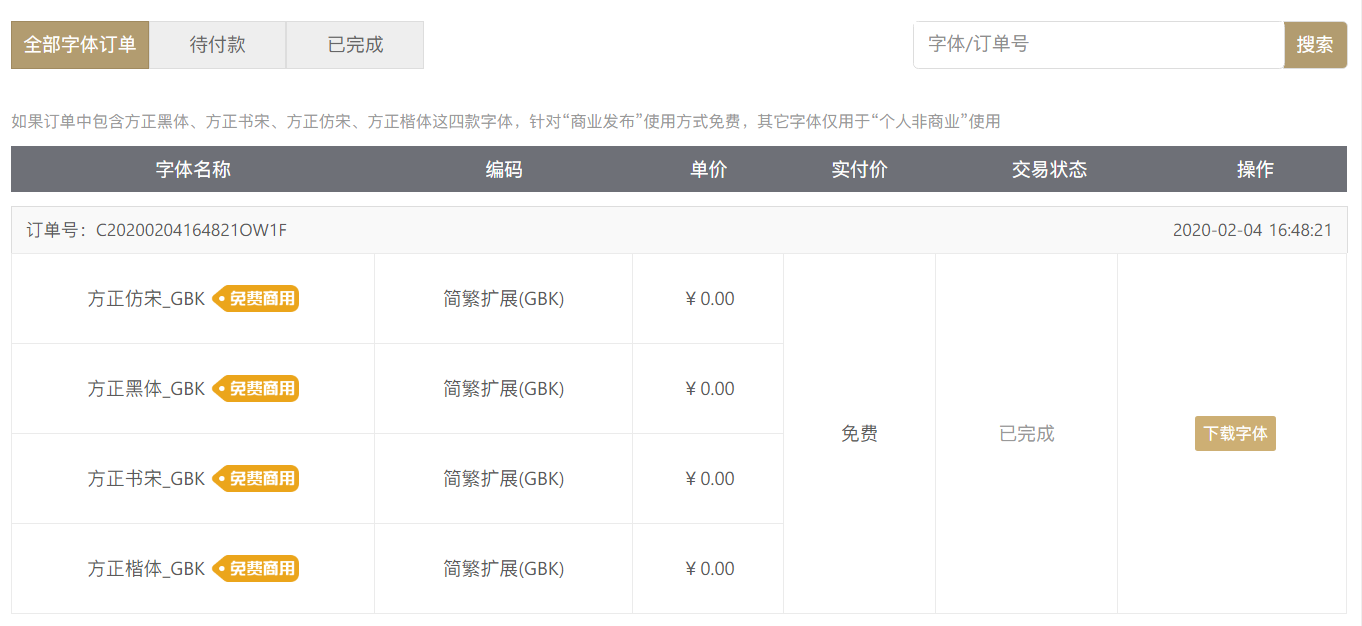
\includegraphics[width=0.9\textwidth]{founder.png}
\end{figure}

\subsubsection{其他中文字体}
如果你想完全自定义字体\footnote{这里仍然以方正字体为例。},你可以选择 \lstinline{chinesefont=nofont},然后在导言区设置
\begin{lstlisting}
\setCJKmainfont[BoldFont={FZHei-B01},ItalicFont={FZKai-Z03}]{FZShuSong-Z01}
\setCJKsansfont[BoldFont={FZHei-B01},ItalicFont={FZHei-B01}]{FZHei-B01}
\setCJKmonofont[BoldFont={FZHei-B01},ItalicFont={FZHei-B01}]{FZFangSong-Z02}
\setCJKfamilyfont{zhsong}{FZShuSong-Z01}
\setCJKfamilyfont{zhhei}{FZHei-B01}
\setCJKfamilyfont{zhkai}{FZKai-Z03}
\setCJKfamilyfont{zhfs}{FZFangSong-Z02}
\newcommand*{\songti}{\CJKfamily{zhsong}}
\newcommand*{\heiti}{\CJKfamily{zhhei}}
\newcommand*{\kaishu}{\CJKfamily{zhkai}}
\newcommand*{\fangsong}{\CJKfamily{zhfs}}
\end{lstlisting}


\subsection[颜色主题]{颜色主题\footnote{测试章节脚注。}}

本模板内置 5 套颜色主题,分别是 \textcolor{eblue}{blue}(默认),\textcolor{egreen}{green}, \textcolor{ecyan}{cyan}, \textcolor{sakura}{sakura} 和 \textcolor{black}{black}。如果不需要颜色,可以选择黑色(black)主题。颜色主题的设置方法:
\begin{lstlisting}[frame=none]
  \documentclass[green]{elegantnote}
  \documentclass[color=green]{elegantnote}
  ...
  \documentclass[black]{elegantnote}
  \documentclass[color=black]{elegantnote}
\end{lstlisting}


\subsection{语言模式}

本模板内含两套语言环境,改变语言环境会改变图表标题的引导词(图,表),文章结构词(比如目录,参考文献等),以及定理环境中的引导词(比如定理,引理等)。不同语言模式的启用如下:
\begin{lstlisting}[frame=none]
  \documentclass[cn]{elegantnote}
  \documentclass[lang=cn]{elegantnote}
  \documentclass[en]{elegantnote}
  \documentclass[lang=en]{elegantnote}
\end{lstlisting}

\begin{note}
只有中文模式才可输入中文,如果需要在英文模式下输入中文,可以自行添加 \lstinline{ctex} 宏包\footnote{需要使用 \lstinline{scheme=plain} 选项才不会把标题改为中文。}或者使用 \lstinline{xeCJK} 宏包设置字体。另外如果在笔记中使用了抄录环境(\lstinline{lstlisting}),并且里面有中文字符,请务必使用 \hologo{XeLaTeX} 编译。
\end{note}


\subsection{定理类环境}

此模板采用了 \lstinline{amsthm} 中的定理样式,使用了 4 类定理样式,所包含的环境分别为
\begin{itemize}
  \item \textbf{定理类}:theorem,lemma,proposition,corollary;
  \item \textbf{定义类}:definition,conjecture,example;
  \item \textbf{备注类}:remark,note,case;
  \item \textbf{证明类}:proof。
\end{itemize}

\begin{remark}
在选用 \lstinline{lang=cn} 时,定理类环境的引导词全部会改为中文。
\end{remark}


\section{写作示例}

我们将通过三个步骤定义可测函数的积分。首先定义非负简单函数的积分。以下设 $E$ 是 $\mathcal{R}^n$ 中的可测集。

\begin{definition}[可积性]
设 $ f(x)=\sum\limits_{i=1}^{k} a_i \chi_{A_i}(x)$ 是 $E$ 上的非负简单函数,其中 $\{A_1,A_2,\ldots$, $A_k\}$ 是 $E$ 上的一个可测分割,$a_1,a_2,\ldots,a_k$ 是非负实数。定义 $f$ 在 $E$ 上的积分为 1. 3
\begin{equation}
   \label{inter}
   \int_{E} f dx = \sum_{i=1}^k a_i m(A_i).
\end{equation}
一般情况下 $0 \leq \int_{E} f dx \leq \infty$。若 $\int_{E} f dx < \infty$,则称 $f$ 在 $E$ 上可积。
\end{definition}

一个自然的问题是,Lebesgue 积分与我们所熟悉的 Riemann 积分有什么联系和区别?之后我们将详细讨论 Riemann 积分与 Lebesgue 积分的关系。这里只看一个简单的例子。设 $D(x)$ 是区间 $[0,1]$ 上的 Dirichlet 函数。即 $D(x)=\chi_{Q_0}(x)$,其中 $Q_0$ 表示 $[0,1]$ 中的有理数的全体。根据非负简单函数积分的定义,$D(x)$ 在 $[0,1]$ 上的 Lebesgue 积分为
\begin{equation}\label{inter2}
  \int_0^1 D(x)dx = \int_0^1 \chi_{Q_0} (x) dx = m(Q_0) = 0
\end{equation}
即 $D(x)$ 在 $[0,1]$ 上是 Lebesgue 可积的并且积分值为零。但 $D(x)$ 在 $[0,1]$ 上不是 Riemann 可积的。

\begin{table}[htbp]
  \centering
  \small
  \caption{燃油效率与汽车价格}
    \begin{tabular}{lcc}
    \toprule
                  &       (1)         &        (2)      \\
    \midrule
    燃油效率      &   -238.90***      &      -49.51     \\
                  &    (53.08)        &      (86.16)    \\
    汽车重量      &                   &        1.75***  \\
                  &                   &       (0.641)   \\
    常数项        &  11253.00***      &    1946.00      \\
                  &  (1171.00)        &   (3597.00)     \\
    观测数        &     74            &      74         \\
    $R^2$         &      0.220        &       0.293     \\
    \bottomrule
    \end{tabular}%
  \label{tab:reg}%
\end{table}%

\begin{theorem}[Fubini 定理]\label{thm:fubi}
若 $f(x,y)$ 是 $\mathcal{R}^p\times\mathcal{R}^q$ 上的非负可测函数,则对几乎处处的 $x\in \mathcal{R}^p$,$f(x,y)$ 作为 $y$ 的函数是 $\mathcal{R}^q$ 上的非负可测函数,$g(x)=\int_{\mathcal{R}^q}f(x,y) dy$ 是 $\mathcal{R}^p$ 上的非负可测函数。并且
\begin{equation}\label{eq:461}
  \int_{\mathcal{R}^p\times\mathcal{R}^q} f(x,y) dxdy=\int_{\mathcal{R}^p}\left(\int_{\mathcal{R}^q}f(x,y)dy\right)dx.
\end{equation}
\end{theorem}

\begin{proof}
Let $z$ be some element of $xH \cap yH$.  Then $z = xa$ for some $a \in H$, and $z = yb$ for some $b \in H$. If $h$ is any element of $H$ then $ah \in H$ and $a^{-1}h \in H$, since $H$ is a subgroup of $G$. But $zh = x(ah)$ and $xh = z(a^{-1}h)$ for all $h \in H$. Therefore $zH \subset xH$ and $xH \subset zH$, and thus $xH = zH$.  Similarly $yH = zH$, and thus $xH = yH$, as required.
\end{proof}


回归分析(regression analysis) 是确定两种或两种以上变量间相互依赖的定量关系的一种统计分析方法。根据定理~\ref{thm:fubi},其运用十分广泛,回归分析按照涉及的变量的多少,分为一元回归和多元回归分析;按照因变量的多少,可分为简单回归分析和多重回归分析;按照自变量和因变量之间的关系类型,可分为线性回归分析和非线性回归分析。


\section{协作人员招募}

招募 Elegant\LaTeX{} 的协作人员,没有工资。工作内容:翻译 Elegant\LaTeX{} 系列模板相关的文稿(中翻英),维护模板的 wiki(主要涉及 Markdown),如果有公众号文稿写作经历的话,也可以帮忙写微信稿。本公告长期有效。

目前 ElegantLaTeX 共有 4 名协作人员,分别是
\begin{itemize}
  \item 官方文档翻译: \href{https://github.com/peggy2006xzyz}{YPY};
  \item GitHub 维基维护: \href{https://github.com/izinngo}{Ingo Zinngo}、\href{https://github.com/xiaohao890809}{追寻原风景};
  \item QQ 群管理员: \href{https://github.com/sikouhjw}{Sikouhjw}.
\end{itemize}

在此感谢他们无私的奉献!


\section{致谢}

截止到 2020 年 04 月 12 日,ElegantNote 2.30 版本发布,ElegantNote 模板在 GitHub 上的收藏数(star)达到了 263。在此特别感谢 China\TeX{} 以及 \href{http://www.latexstudio.net/}{\LaTeX{} 工作室}对于本系列模板的大力宣传与推广。如果你喜欢我们的模板,你可以在 GitHub 上收藏(Star)我们的模板。

\begin{figure}[htbp]
  \centering
  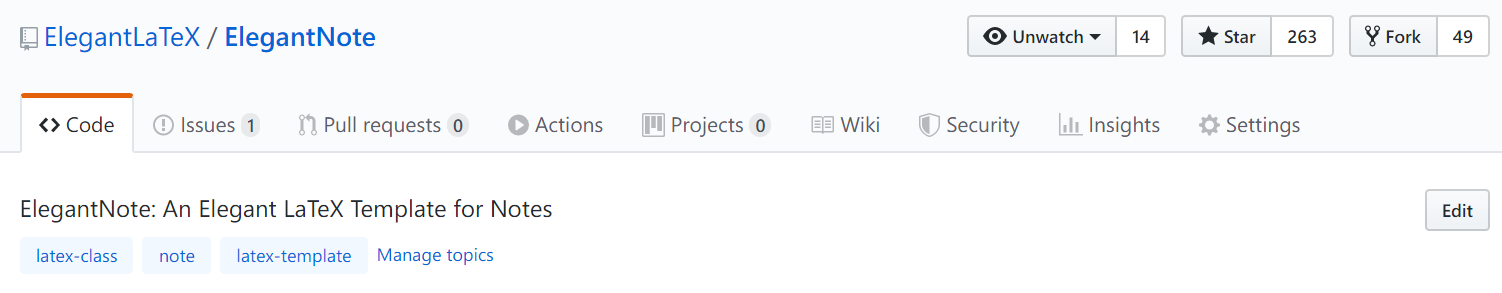
\includegraphics[width=\textwidth]{star.png}
  \caption{一键三连求赞}
\end{figure}

\section{MATLAB代码}

\begin{lstlisting}
% Euler1.m
% Euler method for the ODE model
% u'(t)=t^2+t-u, t \in [0,1]
% Initial condition : u(0)=0 ;
% Exact solution : u(t)=-exp(-t)+t^2-t+1.
clear all
h=0.1;
x=0:h:1;                       % function interval
n=length(x)-1;
u(1)=0;                        % initial value
fun=@(t,u) t.^2+t-u;           % RHS
for i=1:n
    u(i+1)=u(i)+h.*fun(x(i),u(i));
end
ue=-exp(-x)+x.^2-x+1;          % exact solution
plot(x,ue,'b-',x,u,'r+','LineWidth',1.5)
xlabel('x','fontsize', 16), ylabel('y','fontsize',16,'Rotation',0)
legend('Exact ','Numerical','location','North')
title('Euler Method','fontsize',14)
set(gca,'fontsize',14)
\end{lstlisting}



\section{捐赠}

如果您非常喜爱我们的模板,你还可以选择捐赠以表达您对我们模板和我的支持!

\begin{figure}[htbp]
  \centering
  
\includegraphics[width=0.4\textwidth]{donate.jpg}
\end{figure}

\textbf{赞赏费用的使用解释权归 Elegant\LaTeX{} 所有,并且不接受监督,请自愿理性打赏}。10 元以上的赞赏,我们将列入捐赠榜,并且发放捐赠纪念证(全部),谢谢各位金主!

\begin{table}[htbp]
  \scriptsize
  \centering
  \caption{Elegant\LaTeX{} 系列模板捐赠榜}
    \begin{tabular}{*{8}{>{\scriptsize}c}}
    \toprule
    \textbf{捐赠者} & \textbf{金额} & \textbf{时间} & \textbf{渠道} & \textbf{捐赠者} & \textbf{金额} & \textbf{时间} & \textbf{渠道} \\
    \midrule
    Lerh  & 10 RMB & 2019/05/15 & 微信    & 越过地平线 & 10 RMB & 2019/05/15 & 微信 \\
    银桑    & 20 RMB & 2019/05/27 & 微信    & *空    & 10 RMB & 2019/05/30 & 微信 \\
    latexstudio.net & 666 RMB & 2019/06/05 & 支付宝   & A*n   & 40 RMB & 2019/06/15 & 微信 \\
    * 夏   & 22 RMB & 2019/06/15 & 微信    & * 倩   & 21 RMB  & 2019/06/15 & 微信 \\
    Cassis & 11 RMB & 2019/06/30 & 微信    & *君    & 10 RMB & 2019/07/23 & 微信 \\
    P*u   & 50 RMB & 2019/07/30 & 微信    & *萌    & 19 RMB & 2019/08/28 & 微信 \\
    曲豆豆   & 10 RMB & 2019/08/28 & 微信    & 李博    & 100 RMB & 2019/10/06 & 微信 \\
    Njustsll & 10 RMB & 2019/10/11 & 微信    & 刘志阔   & 99.99 RMB & 2019/10/15 & 支付宝 \\
    * 韬   & 16 RMB & 2019/10/17 & 微信    & 赤霓    & 12 RMB & 2019/10/17 & 支付宝 \\
    追寻原风景 & 10 RMB & 2019/10/28 & 微信    & 郭德良   & 88 RMB & 2019/11/03 & 微信 \\
    自强不息  & 20 RMB & 2019/11/04 & 支付宝   & 读书之虫  & 20 RMB & 2019/11/18 & 微信 \\
    *等    & 10 RMB & 2019/11/18 & 微信    & *哲    & 20 RMB & 2019/11/18 & 微信 \\
    佚名    & 10 RMB & 2019/11/24 & 微信    & Jiye Qian & 66 RMB & 2019/12/04 & 微信 \\
    * 阳   & 20 RMB & 2019/12/05 & 微信    & Catcher & 11 RMB & 2019/12/08 & 支付宝 \\
    希尔波特门徒 & 10 RMB & 2019/12/09 & 支付宝   & * 伟   & 10 RMB & 2019/12/09 & 微信 \\
    Simon & 20 RMB & 2019/12/11 & 支付宝   & 流殇丶浅忆 & 66.60 RMB & 2019/12/18 & 支付宝 \\
    羽     & 10 RMB & 2019/12/20 & 支付宝   & * 琛   & 15 RMB & 2019/12/20 & 微信 \\
    随风    & 20 RMB & 2019/12/27 & 支付宝   & Ws    & 23.30 RMB & 2019/12/28 & 微信 \\
    初八    & 100 RMB  & 2020/01/02 & 支付宝   & p*e   & 20 RMB & 2020/01/03 & 微信 \\
    Shunmx & 100 RMB & 2020/01/03 & 微信    & hj    & 10 RMB & 2020/01/03 & 微信 \\
    F*5   & 10 RMB & 2020/01/03 & 微信    & S*m   & 20.20 RMB & 2020/01/03 & 微信 \\
    二代青雉  & 13 RMB & 2020/01/14 & 支付宝   & *?    & 66 RMB & 2020/01/15 & 微信 \\
    Mr. Xiong & 20 RMB & 2020/01/17 & 微信    & *博    & 15 RMB & 2020/01/18 & 微信 \\
    * 者  & 10 RMB & 2020/02/02 & 微信    & Jackie  &  88.80 RMB  &  2020/02/09 & 微信 \\
    Henry\_Sun、 & 50 RMB & 2020/02/14 & 支付宝 & * 桥  & 50 RMB & 2020/02/21 & 微信 \\
    昀琏 & 10 RMB & 2020/03/02 & 支付宝 & S*y  &  10 RMB  &  2020/03/15 & 微信 \\
    * 哥  & 66.66 RMB & 2020/03/17 & 微信    &   K*e & 30 RMB & 2020/03/30 & 微信\\
    * 阳  &  20 RMB  &  2020/04/02 & 微信 & 士*n  & 30 RMB & 2020/04/11 & 微信 \\
    \bottomrule
    \end{tabular}%
  \label{tab:donation}%
\end{table}%


\section{常见问题 FAQ}

\begin{enumerate}[label=\arabic*).]
  \item \textit{如何删除版本信息?}\\
    导言区不写 \lstinline|\version{x.xx}| 即可。
  \item \textit{如何删除日期?}\\
    与版本 \lstinline{\version} 不同的是,导言区不写或注释 \lstinline{\date} 的话,仍然会打印出当日日期,原因是 \lstinline{\date} 有默认参数。如果不需要日期的话,日期可以留空即可,也即 \lstinline|\date{}|。
  \item \textit{如何获得中文日期?}\\
    为了获得中文日期,必须在中文模式下,使用 \lstinline|\date{\zhdate{2019/12/09}}|,如果需要当天的汉化日期,可以使用 \lstinline|\date{\zhtoday}|,这两个命令都来源于 \href{https://ctan.org/pkg/zhnumber}{\lstinline{zhnumber}} 宏包。
  \item \textit{如何添加多个作者?}\\
    在 \lstinline{\author} 里面使用 \lstinline{\and},作者单位可以用 \lstinline{\\} 换行。
    \begin{lstlisting}
      \author{author 1\\ org. 1 \and author 2 \\ org. 2 }
    \end{lstlisting}
\end{enumerate}

\end{document}
